\documentclass[12pt, a4paper, oneside]{ctexbook}
\usepackage{amsmath, amsthm, amssymb, bm, wallpaper}
\usepackage{graphicx, hyperref, mathrsfs, caption}
\usepackage{float, subfigure, enumerate, ulem, paralist}
\usepackage{cite}

\CTEXsetup[format={\Large\bfseries}]{section}
\linespread{1.5}
\newtheorem{theorem}{定理}[section]
\newtheorem{definition}[theorem]{定义}
\newtheorem{lemma}[theorem]{引理}
\newtheorem{corollary}[theorem]{推论}
\newtheorem{example}[theorem]{例}
\newtheorem{proposition}[theorem]{命题}

\newcommand\zm[2]{\begin{proof}[\textbf{#1}]
    #2
\end{proof}}
\newcommand\jie[2]{\begin{proof}[\textbf{#1}]
    #2
\end{proof}}
\newcommand\bv[1]{\boldsymbol{#1}}
\newcommand\mb[1]{\mathbb{#1}}
\newcommand\mc[1]{\mathcal{#1}}

% \renewcommand{\qedsymbol}{}

\captionsetup{labelformat=default,labelsep=space} %去除冒号

\begin{document}

\title{{\Huge{\textbf{非参数统计分析}}\\}}
\author{Lollins}
\date{\today}

\maketitle

\pagenumbering{roman}
\setcounter{page}{1}

\begin{center}
    \Huge\textbf{前言}
\end{center}
\par 记点非参数统计分析的笔记。


\begin{flushright}
    \begin{tabular}{c}
        Lollins \\
        \today
    \end{tabular}
\end{flushright}

\newpage
\pagenumbering{Roman}
\setcounter{page}{1}
\tableofcontents
\newpage
\setcounter{page}{1}
\pagenumbering{arabic}

\chapter{绪论}
\section{序}
\subsection{非参数统计概念及学习意义}
\subsubsection{1、意义}
\subsubsection{2、概念}
\begin{itemize}
    \item \textbf{参数统计方法:}数据样本被视为从分布族的某个参数族抽取出来的总体的代表,
          未知的仅仅是总体分布具体数值,这样推断问题就转化为分布族的若干未知参数的估计问题,
          用样本来对这些参数进行估计或进行假设检验,从而得知背后的分布,这类推断方法称为参数
          统计方法。
    \item \textbf{非参数统计方法:}不假定总体分布的具体形式,尽量从数据(或样本)本身获得所需要的信息,
          通过估计而获得分布的结构,并逐步建立对事物的数学描述和统计模型的方法。
\end{itemize}

\subsection{非参数统计的历史及发展}
\newpage

\section{引言}
\subsection{参数统计方法与非参数统计方法的区别}
\begin{itemize}
    \item \textbf{参数统计方法:}假定总体的分布形式,既利用样本的数据信息,又利用产生数据总体的信息,是一个有效的数据
          分析方法,针对性强,但可能出现大的错误。
    \item \textbf{非参数统计方法:}不假定总体的分布形式,更接近大多数实际情况,故不会出现大的错误。
\end{itemize}

\subsection{非参数统计方法的特点}

\begin{enumerate}[(1)]
    \item 有广泛的适用性(广)
    \item 样本方法是非参数统计的基本方法(样本)
    \item 计算简单(简)
    \item 良好的稳定性(稳)
\end{enumerate}

\chapter{描述性统计}
\begin{definition}[描述性统计]
    是在对产生数据的总体的分布不作任何假设的情况下,整理数据、
    显示数据、分析数据,将数据中有用的信息提取出来的统计方法。
    本章介绍常用的描述性统计方法:\textbf{表格法、图形法和数值方法}。
\end{definition}

\section{图表法}
表格法、图形法描述统计数据主要是频数(率)分布表和直方图。

\section{数值方法}
数值方法主要是用数值来表示数据的中心位置和离散程度等的方法。

\subsection{表示中心位置的数值}
我们要求数据的中心位置满足这样一个\textbf{条件:}它到各个数据点的距离的和比较小。
表示中心位置的数值有平均数、中位数、众数、切尾平均数。

\subsubsection{1、平均数}
如果用平方值距离法,则点a到各数据点$x_1,x_2,...,x_n$的距离的和可以用
$\sum_{i=1}^{n}(x_i-a)^2$来衡量。平均数$\bar{x} = \frac{\sum_{i=1}^{n}x_i}{n}$满足条件:
\begin{equation}
    \sum_{i=1}^n\left(x_i-\bar{x}\right)^2=\min_a\sum_{i=1}^n\left(x_i-a\right)^2
\end{equation}
上式表示\textbf{平均数这一点到各个数据点的平方值距离和最短}。所以在\textbf{平方值距离方法下},数据中心位置的代表是\textbf{平均数}。

\subsubsection{2、中位数}
如果用绝对值距离法,则点a到各数据点$x_1,x_2,...,x_n$的距离的和可以用$\sum_{i=1}^{n}|x_i-a|$
来衡量,中位数me满足条件:
\begin{equation}
    \sum_{i=1}^n|x_i-\max|=\min_a\sum_{i=1}^n|x_i-a|
\end{equation}
上式表示\textbf{中位数这一点到各个数据点的绝对值距离和最短}。所以在\textbf{绝对值距离方法下},数据中心位置的代表是\textbf{中位数}。

\textbf{注:}
\begin{itemize}
    \item 中位数是非线性规划选址问题的解;
    \item 中位数不受极大(小)的影响,有时能较好地表示数据的中心位置。
\end{itemize}

\subsubsection{3、众数}
众数:一组数据中出现频数最高的数据。

\textbf{注:}
\begin{itemize}
    \item 众数也能描述数据的中心位置。特别是定性数据;
    \item 一组数据有偏时,若数据右偏(Positively Skewed),通常有$\bar{x} < me < mo$,
          若数据左偏(Negatively Skewed),通常有$mo < me < \bar{x}$,见图\ref{im2_1}。
\end{itemize}

\begin{figure}
    \centering
    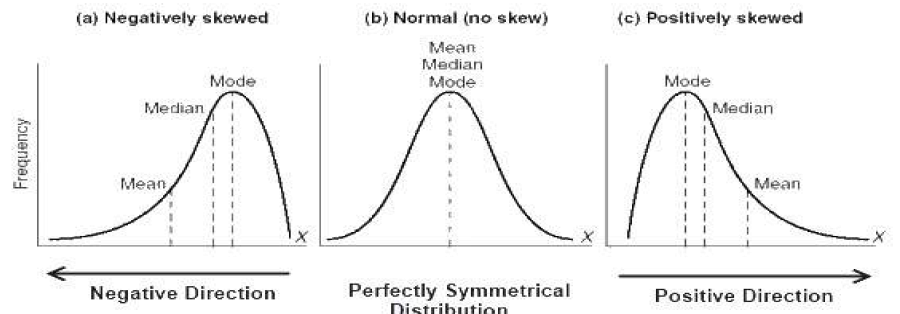
\includegraphics[scale = 0.6]{img/2_1.png}
    \caption{}
    \label{im2_1}
\end{figure}

\subsubsection{4、切尾平均数}
设$X_{(1)},...,X_{(n)}\text{是来自总体X的简单随机样本}X_{1},...,X_{n}$的次序统计值,称
\begin{equation}
    T_{nk}=\frac{1}{n-2k}(x_{(k+1)}+\ldots+x_{(n-k)})
\end{equation}
为原样本的的切尾均值。

\subsection{表示离散程度的数值}
样本方差、标准差、全距(范围)、四分位数间距。

\subsection{标准误}
\begin{equation}
    se = \frac{s}{\sqrt{n}},s\text{为样本方差}
\end{equation}

\subsection{偏度}
偏度反映单峰分布对称性,常用$\beta_s$表示总体偏度,
\begin{equation}
    \beta_s=E[(\frac{x-\mu}\sigma)^3]=\frac{\mu_3}{\sigma^3},\text{其中}\mu_3=E(x-\mu)^3
\end{equation}

\textbf{注:}对称分布的偏度$\beta_s=0$;反之不成立,即$\beta_s=0$,不一定是对称分布。

样本偏度用$b_s$表示,
\begin{equation}
    b_s=\frac{m_3}{m_2^{\frac{3}{2}}},\text{其中}m_j=\frac{1}{n}\sum_i(x_i-\overline{x})^j
\end{equation}

\textbf{注:}$b_s>0$时,倾向于认为数据分布右偏;$b_s<0$时,倾向于认为数据分布左偏;
$b_s\approx 0$时,倾向认为数据分布是对称的。

\subsection{峰度}
峰度反映分布峰的尖峭程度,常用$\beta_k$表示总体峰度。
\begin{equation}
    \beta_k=E[(\frac{x-\mu}{\sigma})^4]=\frac{\mu_4}{\sigma^4}
\end{equation}

\textbf{注:}若$X\sim N(\mu,\sigma^2)$,则$\beta_k=3$。当$\beta_k>3$时,该分布具有过度的峰度,
当$\beta_k<3$时,该分布具有不足的峰度,

样本峰度用$b_k$表示,
\begin{equation}
    b_k=\frac{m_4}{(m_2)^2}
\end{equation}



\begin{thebibliography}{3}
    \bibitem{ref1}孙山泽.非参数统计讲义.北京大学出版社
    \bibitem{ref2}陈希孺.非参数统计.中国科学技术大学出版社
    \bibitem{ref3}李裕奇.非参数统计方法.西南交通大学出版社
\end{thebibliography}

\end{document}